\documentclass{article}

\include{journal_definitions}
\usepackage[a4paper]{geometry}
\usepackage{hyperref}
\usepackage{graphicx}
\usepackage[utf8]{inputenc}
\renewcommand{\figurename}{Figura}

\title{Como ver o invisible}
\author{Pablo Lemos}

\begin{document}
\maketitle

Seguro que algunha vez escoitaches falar da materia escura. Pode que incluso escoitaras 
que só sabemos de que está feito aproximadamente un cinco por cento do Universo, e 
que miraras algunha gráfica como a da figura \ref{fig:piechart}, que amosa a nosa 
ignorancia sobre o outro $95 \%$. É verdade: a maioría do Universo confórmano cousas que non 
coñecemos nin entendemos. E, se o pensas ben, ten moito sentido. Estamolo a observar dende 
un pequeno planeta que dá voltas ao redor dunha pequena estrela, a cal, ás súa vez, da voltas dentro 
dunha Galaxia que se move entre outros millóns de galaxias. ¡Non podemos queixarnos de 
que dende o noso planeta só teñamos acceso unha pequena fracción dos compoñentes do cosmos!

\begin{figure}[h]
\includegraphics{piechart.pdf}
\caption{Esta figura representa os distintos compoñentes do Universo. En azul claro están 
os átomos, como os que forman todos os elementos que coñecemos. En verde está a materia 
escura, e en azul, a enerxía escura. Non sabemos en que consisten ningún dos dous. 
Imaxe: \url{https://wmap.gsfc.nasa.gov/universe/uni_matter.html}
\label{fig:piechart}
}
\end{figure}


Pero se algunha vez escoitaches todo isto, e se tes unha mente curiosa, é posible que 
pensaras: ¿Como sabemos de que está feito o Universo? ¿De onde saen eses números? 
¿Acaso os científicos inventamos ese $4.6 \%$ para que nos sigan pagando? Evidentemente, non. 
Esas preguntas e outras similares son as que intenta responder o campo da cosmoloxía. 
E se o que estás a pensar é que debe ser difícil responder esas preguntas, tes toda a razón. 
De feito, é tan difícil que a cosmoloxía non existiu como disciplina científica ata hai un 
século, cando Einstein publicou a súa teoría da relatividade, a cal tiña como obxectivo describir 
as leis que rexen todo o cosmos. 

Dende entón, pouco a pouco, comezamos a descifrar o enigma das estrelas. Démonos conta de 
que moitos dos puntos brillantes que vemos pola noite non son estrelas, senón galaxias con 
centos de millóns de estrelas cada una. Démonos conta de que, pouco a pouco, esas galaxias se están a afastar da nosa, e que dentro de millóns de anos non poderemos velas. E démonos conta de 
que a maior parte da materia do Universo non se pode ver (de aí o nome `materia escura'). E se estás pensando, mentres les isto, que é todo mentira, que soa a novela de ciencia ficción, 
neste artigo vou tratar de convencerte de que a materia escura é real. E vou tratar de convencerte 
da forma máis eficaz posible: vouche ensinar a materia escura. 

¿Como vou facer iso? ¿Como pretendo ensinarte o invisible? Se o pensas, é lóxico: vou usar lentes. 
¿Que pasa cando ves unha imaxe a través dunha lente? A lente distorsiona a imaxe, ás veces faina 
parecer máis grande ou pequena, outras veces estira a imaxe nunha certa dirección. Se observamos 
unha galaxia moi lonxe, a materia escura que está entre nós e a galaxia distorsiona a imaxe que 
vemos, igual que farían unhas lentes de tamaño cósmico.

\begin{figure}[h]
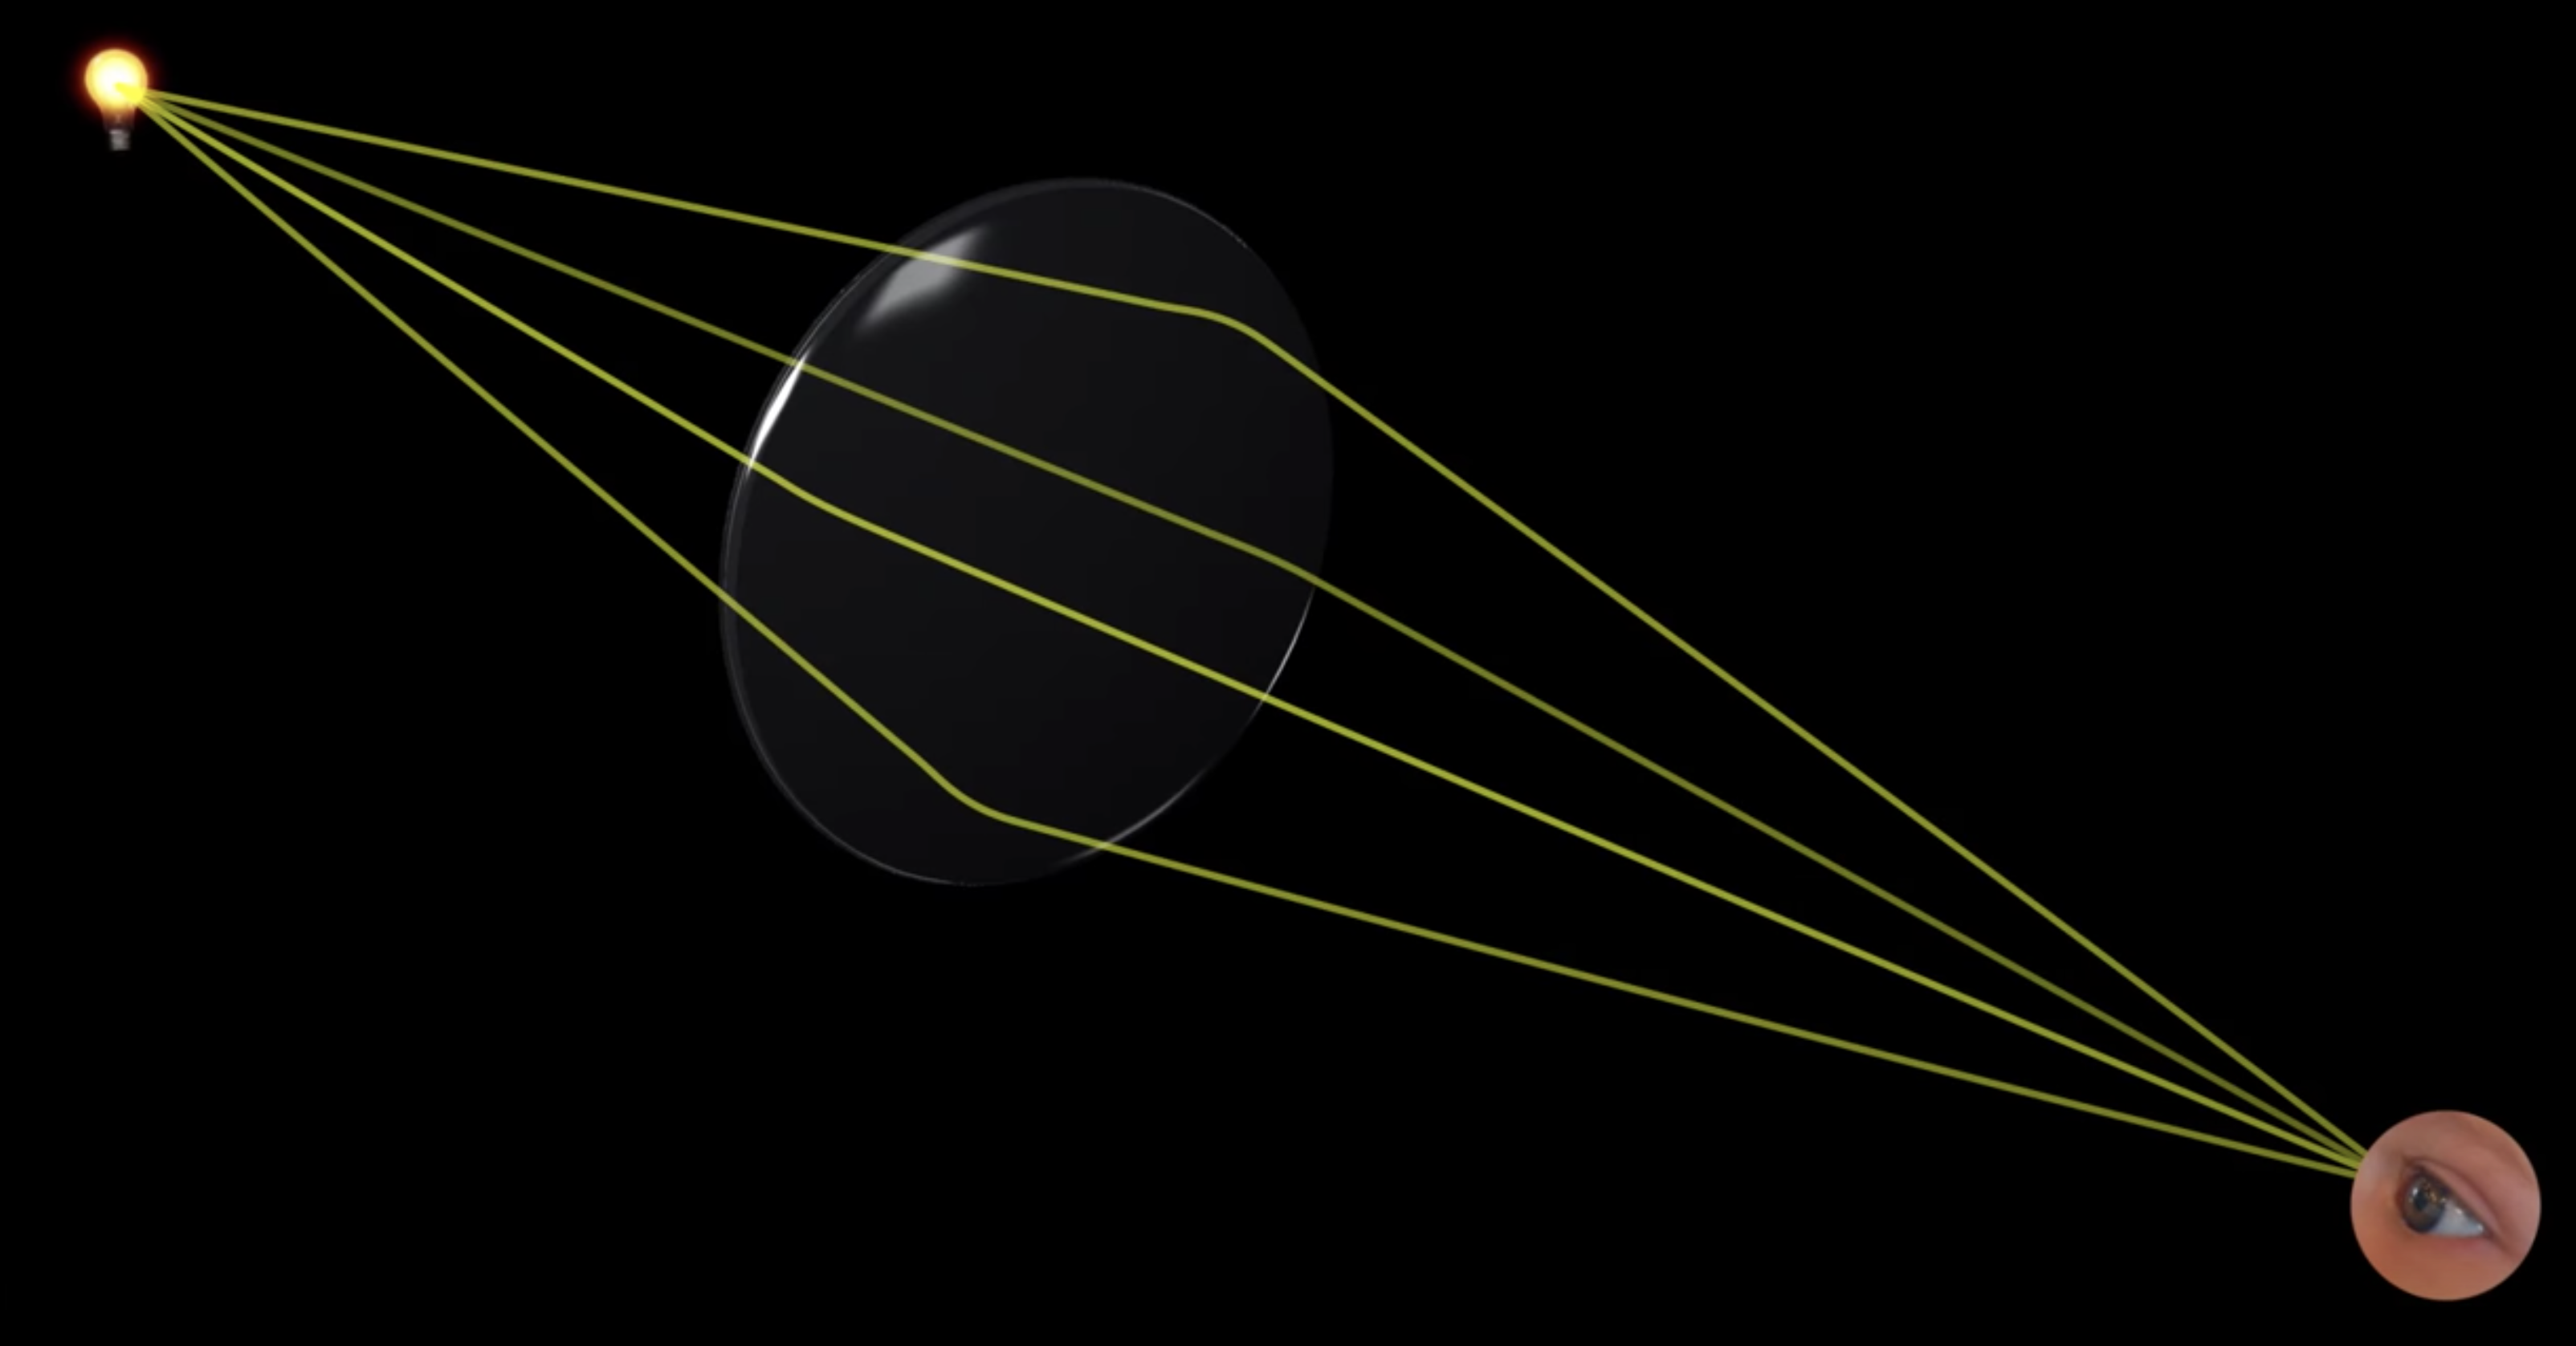
\includegraphics[width=0.49  \textwidth]{lens1}
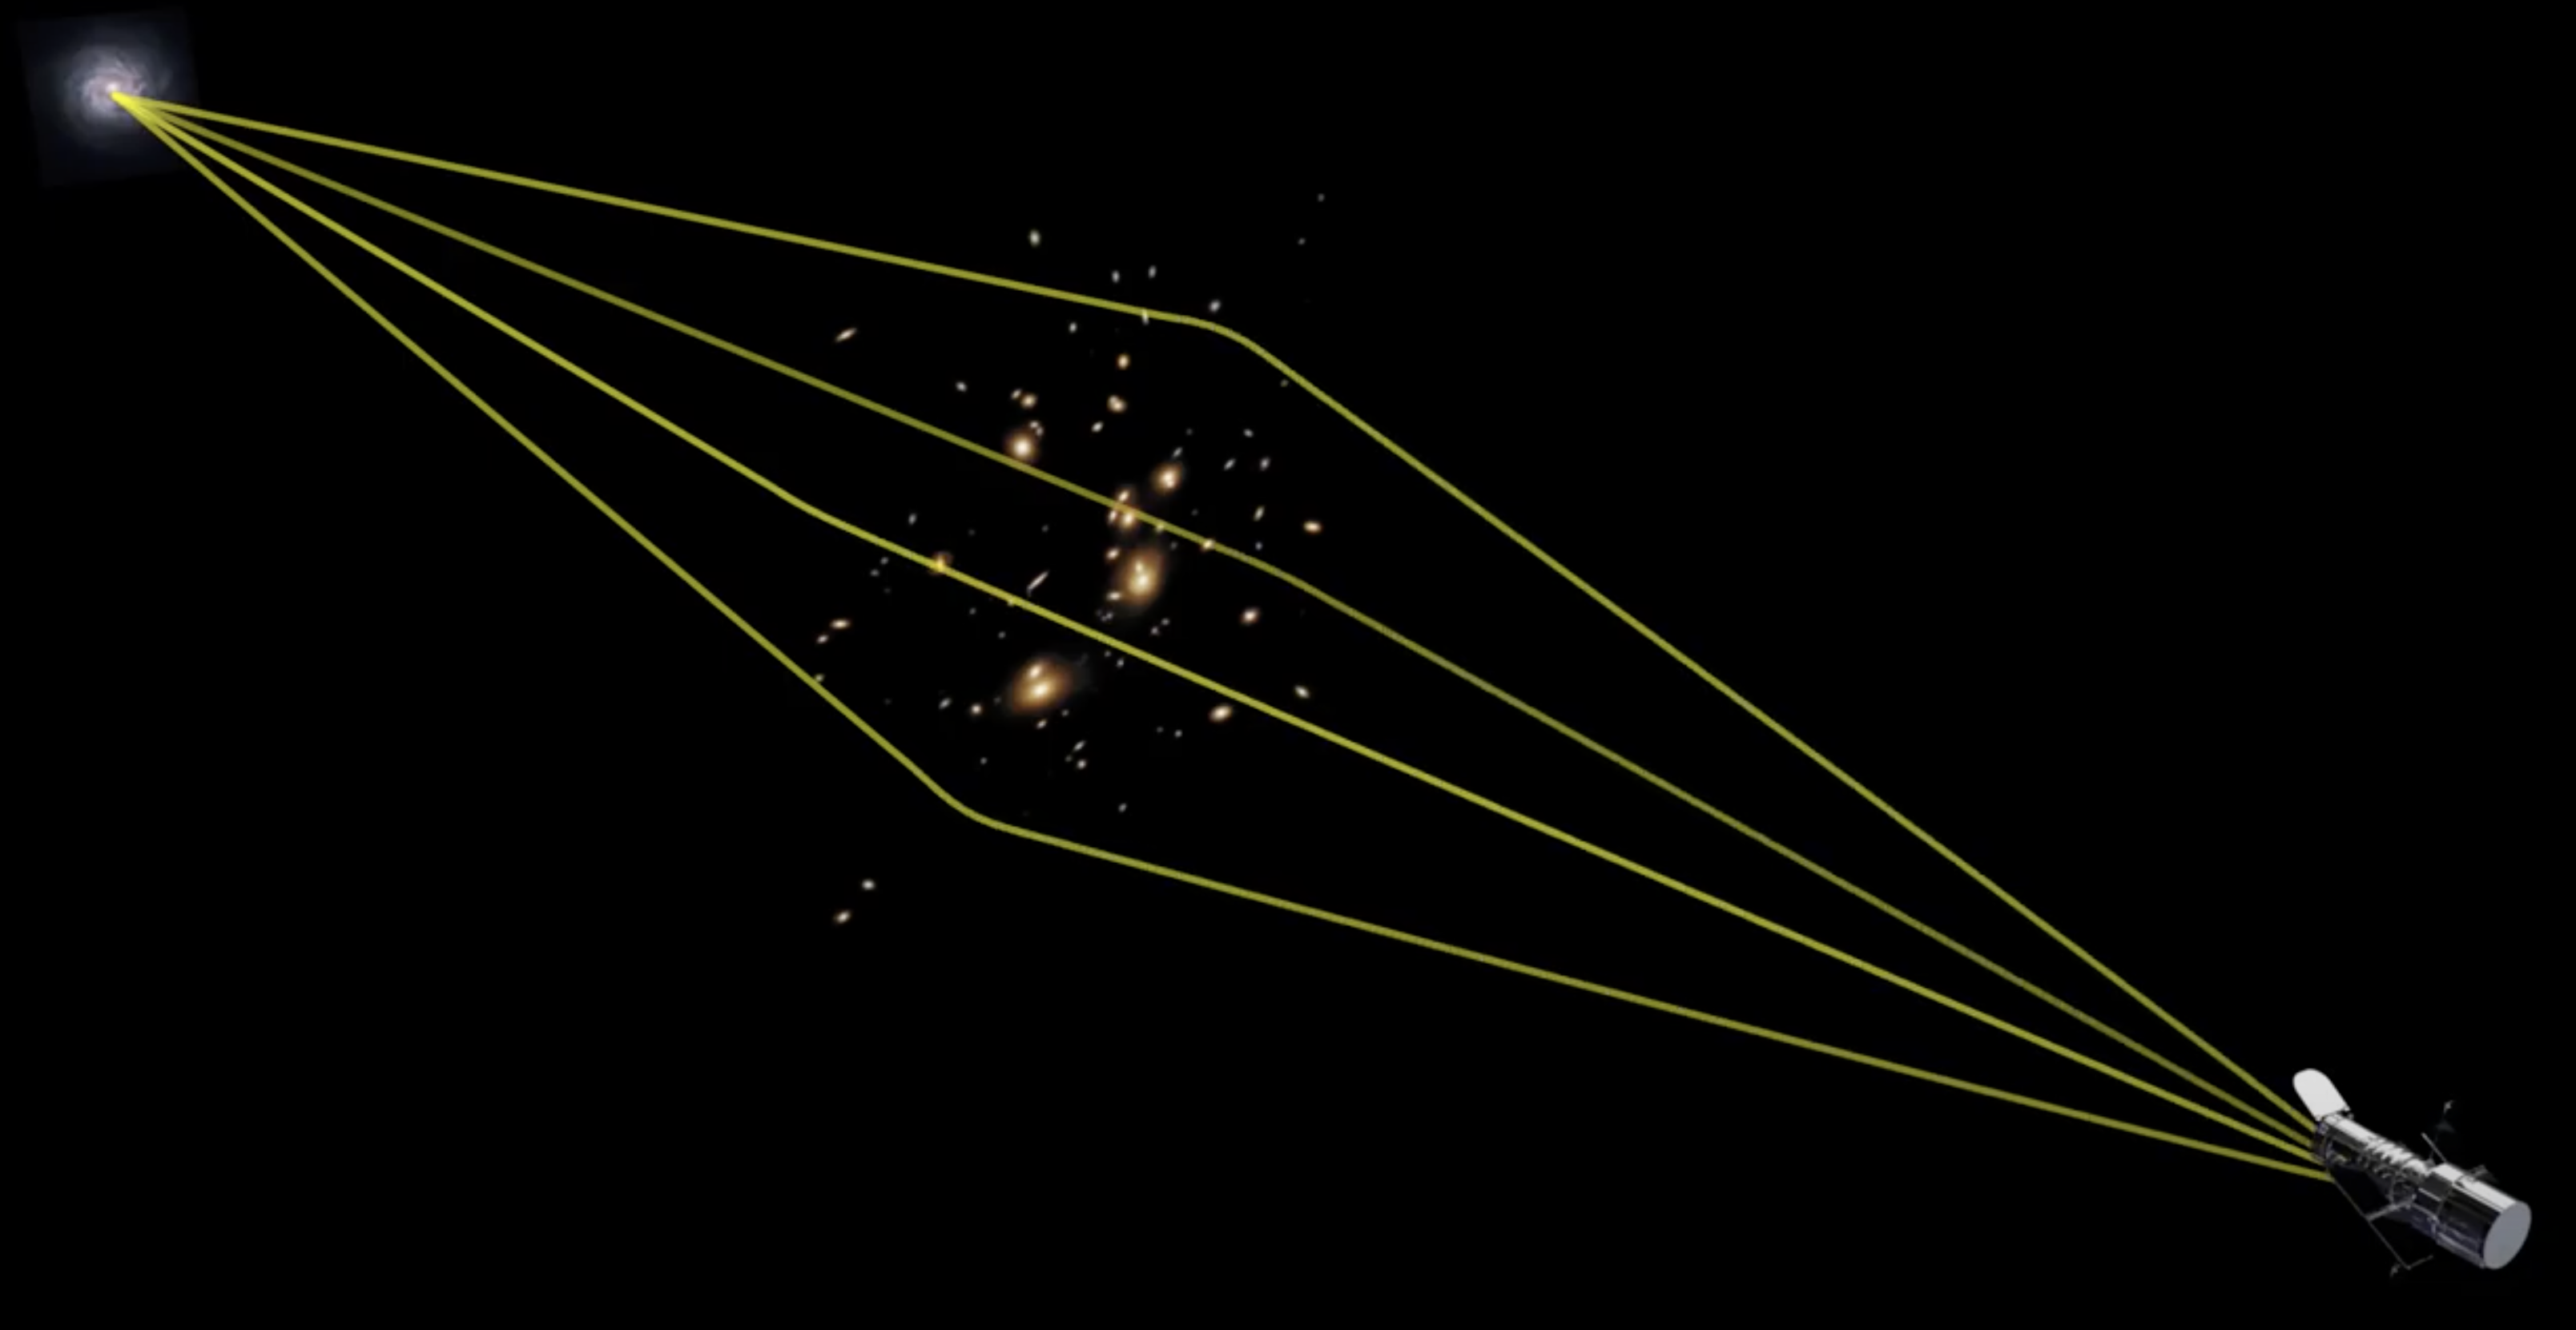
\includegraphics[width=0.49\textwidth]{lens2}
\caption{Ilustración do `efecto lente'. Na esquerda vemos como funciona unha lente de verdade, como 
as que usamos no día a día, cambiando o camiño que segue a luz de camiño aos nosos ollos, e de esta forma 
distorsionando a imaxe. Na dereita vemos como a materia escura fai o mesmo con imaxes de galaxias, 
distorsionándoas no seu camiño cara ao telescopio. Imaxe: {\it Hubble Space Telescope}, \url{https://hubblesite.org/}
\label{fig:lens_example}
}
\end{figure}

Polo tanto, a pesar de que non podemos ver a materia escura directamente, podemos vela indirectamente, 
a través deste `efecto lente' (en inglés {\it lensing}, derivado da palabra {\it lens}, que significa 
lente), ilustrado na figura \ref{fig:lens_example}. Porén, hai outro problema. Se as galaxias foran esferas perfectas, coma un balón de fútbol, sería moi fácil saber como de distorsionadas están. Pero en realidade, a maioría das galaxias son elípticas, coma un ovo. Polo tanto, cando usamos un telescopio e 
vemos unha galaxia que parece estar `estirada', é imposible saber se está estirada porque a estamos a mirar a través 
dunha lente de materia escura ou porque esa é a súa forma real. A solución a este problema 
é mirar non só para unha, senón para millóns de galaxias. Se varias galaxias próximas están alongadas na mesma 
dirección, é moi pouco probable que, por casualidade, todas teñan a mesma forma e apunten ao mesmo sitio.
Nese caso, saberemos que estamos a observar esas galaxias a través dunha lente. E, polo tanto, que estamos vendo, indirectamente,  a invisible materia escura.

Na última década foi posible observar o ceo como nunca antes, grazas a grandes avances tecnolóxicos e 
científicos, e a importantes inversións por parte de gobernos de varios países. Un exemplo disto é a {\it Dark 
Energy Survey}, abreviado como DES, unha colaboración de varias institucións académicas en múltiples países, incluidas
varias españolas, que utilizou o Telescopio Víctor Manuel Blanco en Chile para observar aproximadamente 300 millóns de galaxias, empregando 
unha técnica chamada fotometría. Grazas á gran cantidade de imaxes obtidas e aos avanzados métodos estadísticos empregados, DES 
logrou, entre outras cosas, crear un mapa da materia escura vista dende a nosa galaxia. O mapa da figura
 \ref{fig:massmap} amosa a cantidade de materia escura que hai en diferentes direccións do ceo. As zonas azuis son áreas 
 con menos materia escura, e as zonas vermellas, con máis. Seguro que se estás vendo esta imaxe, recordarache a algo, 
 como cando ves as nubes e buscas formas. Moita xente pensa nunha arañeira. Por iso, coloquialmente, chamámoslle a 
 arañeira cósmica ({\it cosmic web} en inglés). 

Nos próximos anos, telescopios aínda máis potentes que DES mellorarán estas primeiras imaxes da materia escura, 
observando moitas máis galaxias con superior precisión. O noso obxectivo segue sendo descubrir de que está feito 
este misterioso e invisible compoñente do Universo, que é moito máis común que a materia que coñecemos. Quizais 
algún día, dende o noso pequeno planeta, poidamos descifrar de que está feito o Universo. De momento, por primeira 
vez, podemos ver o invisible. 

\begin{figure}[h]
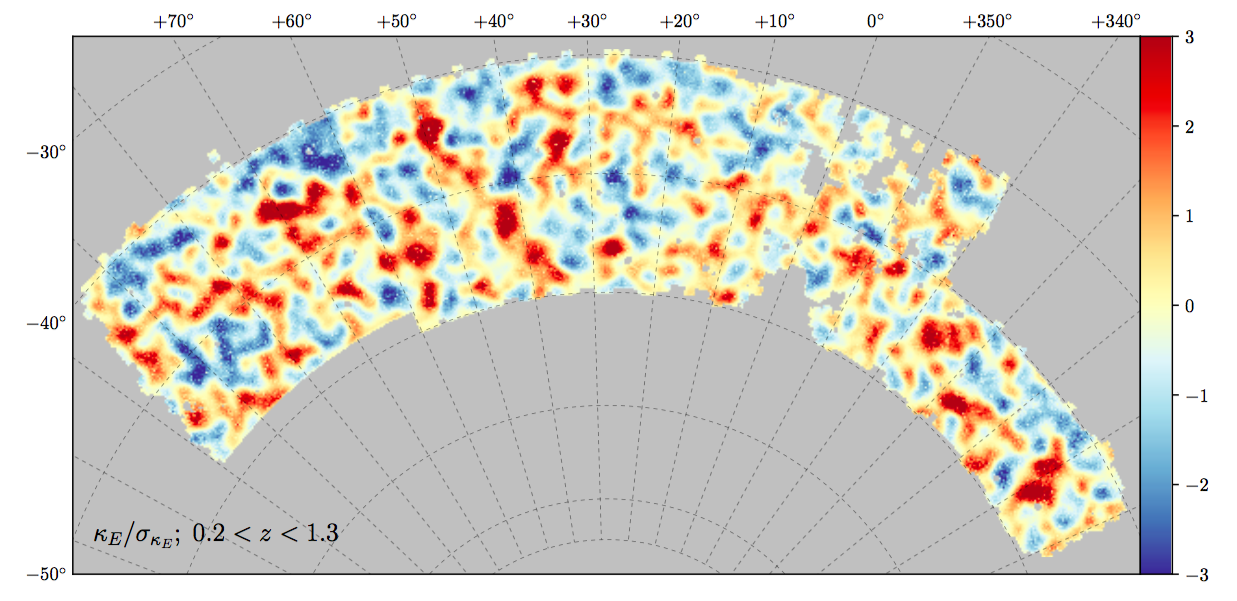
\includegraphics[width=\textwidth]{Y1-massmap}
\caption{Mapa da materia escura observado por DES. Imaxe: \cite{chang}.
\label{fig:massmap}
}
\end{figure}

\bibliographystyle{apalike}
\bibliography{ag}

\end{document}
